% This is samplepaper.tex, a sample chapter demonstrating the
% LLNCS macro package for Springer Computer Science proceedings;
% Version 2.20 of 2017/10/04
%
\documentclass[runningheads]{llncs}
%
\usepackage{graphicx}
% Used for displaying a sample figure. If possible, figure files should
% be included in EPS format.
%
% If you use the hyperref package, please uncomment the following line
% to display URLs in blue roman font according to Springer's eBook style:
% \renewcommand\UrlFont{\color{blue}\rmfamily}

\begin{document}
%
\title{DM1\thanks{Supported by organization x.}}
%
%\titlerunning{Abbreviated paper title}
% If the paper title is too long for the running head, you can set
% an abbreviated paper title here
%
\author{Tim Mooren\inst{1}\orcidID{11710160} \and
Second Author\inst{1}\orcidID{1111-2222-3333-4444} \and
Third Author\inst{1}\orcidID{2222--3333-4444-5555}}
%
\authorrunning{F. Author et al.}
% First names are abbreviated in the running head.
% If there are more than two authors, 'et al.' is used.
%
\institute{Vrije Universiteit Amsterdam, The Netherlands}
%
\maketitle              % typeset the header of the contribution
%
\begin{abstract}
The abstract should briefly summarize the contents of the paper in
150--250 words.

\keywords{First keyword  \and Second keyword \and Another keyword.}
\end{abstract}
%
%
%
\section{Task 1: DATA PREPARATION}
\subsection{TASK 1A: EXPLORATORY DATA ANALYSIS}
\subsubsection{Data Properties}
% Notice all sorts of properties of the dataset: how many records are there, how many attributes, what kinds of attributes are there, ranges of values, distribution of values, relationships between attributes, missing values, and so on. A table is often a suitable way of showing such properties of a dataset. Notice if something is interesting (to you, or in general), make sure you write it down if you find something worth mentioning.
There are 376912 entries in the dataset, of which 202 have missing values. All the missing values belong to the variables 'circumplex.arousal' and 'circumplex.valence'. 

Regarding the ranges of the values in the data, it was discovered that the variables 'appCat.builtin' and 'appCat.entertainment' had negative values, which is problematic because they represent a duration and should therefore always be positive. This was solved at the data cleaning stage.

% FALSE:? Moreover, it was discovered that the values for the variables 'sms' and 'call' are always 1 (symbolizing 'yes'). Because the values are always the same, these variables do not provide any information for our model. Thus, it was decided to omit these variables to improve efficiency of the algorithm.

\subsubsection{Plots}
% Make various plots of the data. Is there something interesting worth reporting? Report the figures, discuss what is in them. What meaning do those bars, lines, dots, etc. convey? Please select essential and interesting plots for discussion, as you have limitedspace for reporting your findings.

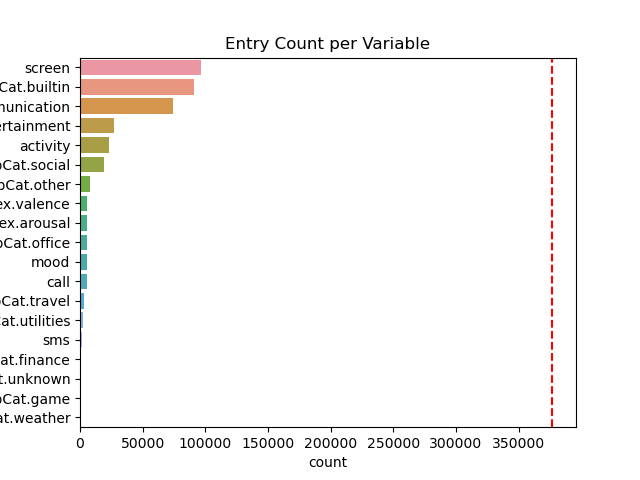
\includegraphics{plots/variable_count.png}


\subsection{TASK 1B: DATA CLEANING}

\subsubsection{Extreme and Incorrect Values}
Through the exploratory data analysis it was discovered that XXXMANY entries contained incorrect values. Entries where variables had negative values for duration were removed.


\subsubsection{Imputation}
The missing values from variables 'circumplex.arousal' and 'circumplex.valence' were imputed using two methods. The first method involved replacing the missing values with the mean of the variable per participant per day. It was decided to use this method rather than the overall mean because it was expected that this would result in a closer approximation to the actual value of those entries.

second method is mean per person. 

\subsection{TASK 1C: FEATURE ENGINEERING}
\subsubsection{Weekdays}
One feature that was added for the purpose of temporal mood prediction is the day of the week, which was constructed from the original data. This might be a valuable feature as it is reasonable that individual's mood may depend on the day of the week. For example, people may be in better mood on Saturday than on Monday.
\subsubsection{Participant's Average Mood}
PARTICPANT'S AVERAGE MOOD CAN BE IMPLEMENTED MAYBE?

\section{TASK 2: CLASSIFICATION }
\subsection{TASK 2A: APPLICATION OF CLASSIFICATION ALGORITHMS}

\subsection{TASK 2B: WINNING CLASSIFICATION ALGORITHMS}









































%
% ---- Bibliography ----
%
% BibTeX users should specify bibliography style 'splncs04'.
% References will then be sorted and formatted in the correct style.
%
% \bibliographystyle{splncs04}
% \bibliography{mybibliography}
%
\begin{thebibliography}{8}
\bibitem{ref_article1}
Author, F.: Article title. Journal \textbf{2}(5), 99--110 (2016)

\bibitem{ref_lncs1}
Author, F., Author, S.: Title of a proceedings paper. In: Editor,
F., Editor, S. (eds.) CONFERENCE 2016, LNCS, vol. 9999, pp. 1--13.
Springer, Heidelberg (2016). \doi{10.10007/1234567890}

\bibitem{ref_book1}
Author, F., Author, S., Author, T.: Book title. 2nd edn. Publisher,
Location (1999)

\bibitem{ref_proc1}
Author, A.-B.: Contribution title. In: 9th International Proceedings
on Proceedings, pp. 1--2. Publisher, Location (2010)

\bibitem{ref_url1}
LNCS Homepage, \url{http://www.springer.com/lncs}. Last accessed 4
Oct 2017
\end{thebibliography}
\end{document}
